% Emerald Publishing - Construction Innovation Submission Template
% by Oleksandr Melnyk
% Ver 0.0.4
% Based on: https://www.emeraldgrouppublishing.com/journal/ci#author-guidelines

\documentclass{article}

\usepackage[english]{babel}

% Set page size and margins
% Replace `letterpaper' with `a4paper' for UK/EU standard size
\usepackage[a4paper,top=2cm,bottom=2cm,left=3cm,right=3cm,marginparwidth=1.75cm]{geometry}

% Useful packages
\usepackage{amssymb}
\usepackage{siunitx}
\PassOptionsToPackage{hyphens}{url}\usepackage{hyperref}
\usepackage{cleveref}
\usepackage[utf8]{inputenc}
\usepackage[right]{lineno}
\usepackage{csquotes}
\usepackage{booktabs}
\usepackage{longtable}
\usepackage{adjustbox}
\usepackage{graphicx}
\usepackage{array}
\usepackage{url}
\usepackage{titlesec}
%\usepackage[compatibility=false]{caption}
\usepackage{authblk}
\usepackage{xcolor} % Load the xcolor package for color options
\renewcommand{\thetable}{\Roman{table}}

% Define a new format for \subsection
\titleformat{\subsection}
  {\mdseries\itshape\large} % Medium series, italic shape, and large font size
  {\thesubsection}{1em}{} % Numbering, spacing, and the section title itself


% Emerald Harvard Citation Style

\usepackage[english]{babel}
\usepackage[style=authoryear,backend=biber,natbib=true,maxcitenames=2,uniquelist=false]{biblatex}
\addbibresource{bibliography.bib} % your .bib file

% Customizing biblatex for Harvard style
\DeclareNameAlias{sortname}{family-given}
\DeclareNameAlias{default}{family-given}

\renewbibmacro{in:}{}
\DeclareFieldFormat[article]{title}{\mkbibquote{#1}\addcomma}
\DeclareFieldFormat[book]{title}{\mkbibemph{#1}\addcomma}
\DeclareFieldFormat[bookinbook]{title}{\mkbibemph{#1}\addcomma}
\DeclareFieldFormat[inbook]{title}{\mkbibquote{#1}\addcomma}
\DeclareFieldFormat[incollection]{title}{\mkbibquote{#1}\addcomma}
\DeclareFieldFormat[inproceedings]{title}{\mkbibquote{#1}\addcomma}
\DeclareFieldFormat[manual]{title}{\mkbibemph{#1}\addcomma}
\DeclareFieldFormat[misc]{title}{\mkbibemph{#1}\addcomma}
\DeclareFieldFormat[thesis]{title}{\mkbibemph{#1}\addcomma}
\DeclareFieldFormat[unpublished]{title}{\mkbibquote{#1}\addcomma}
\DeclareFieldFormat[patent]{title}{\mkbibemph{#1}\addcomma}
\DeclareFieldFormat[report]{title}{\mkbibemph{#1}\addcomma}
\DeclareFieldFormat[online]{title}{\mkbibquote{#1}\addcomma}
\DeclareFieldFormat[software]{title}{\mkbibemph{#1}\addcomma}
\DeclareFieldFormat[booklet]{title}{\mkbibemph{#1}\addcomma}
\DeclareFieldFormat[periodical]{title}{\mkbibemph{#1}\addcomma}
\DeclareFieldFormat[standard]{title}{\mkbibemph{#1}\addcomma}

\DeclareFieldFormat[article]{journaltitle}{\iffieldundef{shortjournal}{\mkbibemph{#1}\addcomma}{\mkbibemph{\printfield{shortjournal}}\addcomma}}
\DeclareFieldFormat{volume}{\bibstring{volume}~#1}
\DeclareFieldFormat{number}{\bibstring{number}~#1}

% Definitions for "Vol." and "No."
\DefineBibliographyStrings{english}{
  volume = {Vol.},
  number = {No.}
}

\renewbibmacro*{volume+number+eid}{%
  \printfield{volume}%
  \setunit*{\addspace}%
  \printfield{number}%
  \setunit{\addcomma\space}%
  \printfield{eid}}

\renewbibmacro*{journal+issuetitle}{%
  \usebibmacro{journal}%
  \setunit*{\addcomma\space}%
  \usebibmacro{volume+number+eid}%
  \setunit{\addcomma\space}%
  \usebibmacro{issue+date}}

\renewbibmacro*{publisher+location+date}{%
  \printlist{publisher}%
  \iflistundef{location}
    {\setunit*{\addcomma\space}}
    {\setunit*{\addcolon\space}}%
  \printlist{location}%
  \setunit*{\addcomma\space}%
  \usebibmacro{date}}

\renewcommand*{\bibpagespunct}{\addcomma\space}

% Customizing page field format to prevent duplication
% \DeclareFieldFormat{pages}{%
%   \mkfirstpage[{\mkpageprefix[page]{#1}}]{#1}}

% Customizing citations for Harvard style
\DeclareCiteCommand{\cite}[\mkbibparens]
  {\usebibmacro{prenote}}
  {\usebibmacro{citeindex}%
   \usebibmacro{cite}}
  {\multicitedelim}
  {\usebibmacro{postnote}}

\renewbibmacro*{cite:labelyear+extrayear}{%
  \iffieldundef{labelyear}
    {}
    {\printtext[bibhyperref]{%
       \printfield{labelyear}%
       \printfield{extrayear}}}}

\renewbibmacro*{cite:labeldate+extradate}{%
  \iffieldundef{labelyear}
    {}
    {\printtext[bibhyperref]{%
       \printfield{labelyear}%
       \printfield{extradate}}}}

\AtEveryBibitem{
  \clearfield{month}
  \clearfield{day}
  \ifentrytype{book}{
    \clearlist{location}
  }{}
}

% Formatting "et al." in italics followed by a comma
\DefineBibliographyStrings{english}{
  andothers = {\textit{et al.},}
}

\DeclareFieldFormat[article]{volume}{\bibstring{jourvol}\addnbspace #1}
\DeclareFieldFormat[article]{number}{\bibstring{number}\addnbspace #1}
\DeclareFieldFormat[article]{volume}{Vol. #1}
\DeclareFieldFormat[article]{number}{No. #1}
% Customizing DOI field format to lowercase "doi"
%\DeclareFieldFormat{doi}{\bibstring{doi}\addcolon\space\url{#1}}

% Customizing URL field format to "available at:"
\DeclareFieldFormat{url}{\bibstring{available at}\addcolon\space\url{#1}}
\DeclareFieldFormat{urldate}{\mkbibparens{accessed \addspace#1}}

% Customizing urldate to match the required format
\DeclareFieldFormat{urldate}{%
  \mkbibparens{accessed\space%
    \thefield{urlday}\addspace%
    \mkbibmonth{\thefield{urlmonth}}\addspace%
    \thefield{urlyear}}}

% Configure cleveref
\crefformat{figure}{#2Figure~#1#3}
\Crefformat{figure}{#2Figure~#1#3}
\crefformat{table}{#2Table~#1#3}
\Crefformat{table}{#2Table~#1#3}
\crefformat{section}{#2Section~#1#3}
\Crefformat{section}{#2Section~#1#3}

%%% Flags, colors and comments
\definecolor{dkred}{rgb}{.6,0,0}
\definecolor{dkgreen}{rgb}{0,.5,0}
\newif\ifdraft\drafttrue
\newcommand{\displaycomment}[1]{{#1}} % inline
\newcommand\hl[1]{{\color{dkred} #1}}
\newcommand{\alt}{\uparrow}
\newcommand{\olremark}[2]{{\color{dkgreen}(#1: #2)}}
\newcommand{\varemark}[2]{{\color{dkred}(#1: #2)}}
\newcommand{\ftremark}[2]{{\color{teal}(#1: #2)}}
\newcommand{\pfremark}[2]{{\color{blue}(#1: #2)}}
\newcommand{\fsremark}[2]{{\color{violet}(#1: #2)}}
\newcommand{\acremark}[2]{{\color{purple}(#1: #2)}}
\newcommand{\lnegremark}[2]{{\color{cyan}(#1: #2)}}
\newcommand{\loliremark}[2]{{\color{orange}(#1: #2)}}
\ifdraft
\newcommand{\mmerenda}[1]{\varemark{MM}{#1}}
\newcommand{\scolli}[1]{\olremark{SC}{#1}}
\else
\newcommand{\mmerenda}[1]{}
\newcommand{\scolli}[1]{}
\fi

%%%%%%%%%%%%%%%%%%%%%%%%%%%%%%%%%%%%%%%%%%%%%%%%%%%%%%%%%%%%%%%
%Front Matter
\author[1]{Colli Simone}
\author[1]{Merenda Saverio Mattia}

\affil[1]{
    \url{simone.colli@studenti.unipr.it}
    }
\affil[2]{
    \url{saveriomattia.merenda@studenti.unipr.it}
    }

% Titolo
\title{Ottimizzazione dei Garanti accademici}

\begin{document}
\maketitle

%%%%%%%%%%%% TODO list da rimuovere in seguito
\mmerenda{TODO list (da rimuovere piu' avanti)}\\
\mmerenda{
  \begin{itemize}
    \item Modificare il nome del progetto su github e nel container docker
      da pd-project a ottimizzazione-garanti-accademici
  \end{itemize}
}
%%%%%%%%%%%%%%%%%%%%%%%%%%%%%%%%%%%%%%%%% TODO

\begin{abstract}
    Questo lavoro presenta l'analisi e l'implementazione di un sistema automatizzato per 
    l'assegnazione dei garanti ai corsi universitari, in conformità ai requisiti ministeriali. 
    L'obiettivo principale è garantire che ogni corso soddisfi i vincoli minimi di docenza, 
    rispettando le regole di distribuzione tra diverse categorie di docenti e ottimizzando 
    l'uso delle risorse disponibili.

    Utilizzando la programmazione logica con Answer Set Programming (ASP), 
    abbiamo modellato il problema attraverso fatti, regole e vincoli derivati dai dati 
    ministeriali e universitari. Abbiamo implementato una serie di vincoli per rispettare 
    i minimi richiesti di docenti per corso, evitando sovrapposizioni improprie tra gli 
    incarichi dei docenti e considerando scenari realistici in cui un docente può assumere 
    più ruoli parziali.
    
    L'approccio è stato testato su un dataset reale contenente informazioni su corsi, SSD 
    (Settori Scientifico Disciplinari) e docenti dell'Università degli Studi di Parma. 
    I risultati dimostrano come il sistema possa trovare configurazioni ottimali che 
    soddisfano i requisiti, massimizzando l'efficienza e mantenendo flessibilità 
    nell'assegnazione dei docenti.

\end{abstract}
% \linenumbers % utilizzato per debug
\section{Introduzione}
\label{sec:introduction}

L'assegnazione dei garanti nei corsi universitari costituisce una 
questione fondamentale per la gestione ottimale delle risorse accademiche. 
Nell'ambito universitario, il \textit{garante} è un docente responsabile 
di rappresentare e tutelare la qualità didattica di un corso, garantendo 
il rispetto dei requisiti disciplinari e istituzionali. I garanti possono 
appartenere a diverse categorie contrattuali: docenti a tempo indeterminato, 
docenti a tempo determinato e, in casi eccezionali, docenti a contratto.

La sfida principale consiste nel soddisfare i vincoli ministeriali 
relativi ai garanti, garantendo al contempo un'allocazione equilibrata 
e sostenibile delle risorse. Ogni corso deve essere supportato da un 
numero minimo di garanti, suddivisi tra le diverse fasce contrattuali, 
per assicurare un livello adeguato di competenza e rappresentatività. 
Inoltre, è indispensabile che almeno il 50\% dei garanti afferisca al 
Settore Scientifico Disciplinare (SSD) caratterizzante del corso, al 
fine di garantire la coerenza tra l'offerta formativa e le competenze 
disciplinari.

Un'ulteriore complessità è rappresentata dall'impiego di docenti a 
contratto, il cui utilizzo deve essere limitato e subordinato alle 
sole situazioni in cui non sia possibile soddisfare i requisiti 
attraverso i docenti strutturati. La necessità di rispettare questi 
vincoli, combinata con la disponibilità limitata di personale e la 
necessità di bilanciare il carico di lavoro, rende questo problema 
una sfida organizzativa e computazionale significativa.

Un primo ostacolo affrontato in questo progetto riguarda la fase di 
pre-elaborazione dei dati forniti dall'università, descritta nella 
Sezione~\ref{sec:pre-proc} di questo elaborato. I dati risultano 
disomogenei e incompleti, richiedendo una significativa pulizia e 
riorganizzazione prima di poter essere utilizzati efficacemente nel 
modello ASP. Questa fase ha richiesto lo sviluppo di strumenti 
dedicati per uniformare e validare i dati.

La Sezione~\ref{sec:asp} esplora il cuore del nostro approccio, 
ovvero la costruzione del modello ASP. Qui abbiamo implementato 
regole logiche per soddisfare i vincoli ministeriali e massimizzare 
l'efficienza dell'assegnazione dei garanti, tenendo conto delle 
limitazioni sulle fasce contrattuali e sull'impiego dei docenti a contratto.

Successivamente, nella Sezione~\ref{sec:expval}, presentiamo 
i risultati ottenuti su un esempio ridotto, un test che ha permesso 
di validare il modello in un ambiente controllato e di analizzare la qualità 
delle soluzioni generate. Infine, la Sezione~\ref{sec:dataset-tutti-dipartimenti} descrive 
l'applicazione del modello su un dataset completo contenente tutti i corsi 
universitari, eseguendo un benchmark su larga scala per valutare la 
capacità del nostro approccio di risolvere problemi reali e complessi.
\section{Pre processing}
\label{sec:pre-proc}

\scolli{Usa questa macro per scrivere commenti}



I dati analizzati sono stati forniti in formato Excel dall'ufficio xxx\scolli{che ufficio?}
presentando quindi una struttura tabellare composta da una serie di campi.

Per consetire un'analisi efficace e priva di errori è stato necessario effettuare una fase di
preprocessing volto a corregge e migliorare la qualità e coerenza dei dati e a scomporre il dataset.

I file forniti presentano al loro interno:
\begin{itemize}
    \item Docenti e ricercatori.
    \item Coperture degli insegnamenti dei vari corsi di laurea.
\end{itemize}

Dopo un approfondita analisi di questi file abbiamo deciso di considerare rilevanti per l'analisi solo alcuni campi.
Nel file dei docenti abbiamo considerato rilevanti solo le colonne contententi la matricola, la fascia e
il settore scientifico disciplinare (SSD).
Nel file relativo alle coperture abbiamo considerato rilevanti solo le colonne contenenti
la matricola del docente, il codice del tipo di corso, il codice del corso di laurea, il settore scientifico disciplinare (SSD).

Per riuscire ad ottenere i dati sopra descritti ben definiti abbiamo effettuato una serie di operazioni di preprocessing per migliorare la qualità dei
dati, così da facilitare l'automatizzazione del workflow generale.

La maggior parte delle operazioni sono state svolte sul file contentente le coperture degli insegnamenti, e sono raggruppabili nei seguenti macroprocessi:
\begin{itemize}
    \item Gestione delle righe contententi una o più colonne vuote.
    \item Scomposizione dei dataset, suddivisione dei dati in sottoinsiemi più piccoli e gestibili.
    \item Identificazione dei casi particolari in modo univoco ed automatizzato.
\end{itemize}

Le righe completamente vuote sono state rimosse in quanto non rilevanti per l'analisi, e le righe che presentano le colonne relative al docente (matricola, nome e cognome) vuote sono state
isolate all'interno di un file separato in quanto rappresentano degli insegnamenti non assegnati ad alcun docente (`insegnamenti_senza_docente.xlsx`).

A questo punto abbiamo suddiviso i dati in sottoinsiemi più piccoli e gestibili.
Come prima cosa abbiamo suddiviso le righe che presentano gli insegnamenti tenuti dai docenti/ricercatori e gli insegnamenti tenuti dai docenti a contratto.

Per fare ciò abbiamo sfruttato il file dei docenti che ci è stato fornito, utilizzato la colonna contentente la matricola per identificare ed estrarre, in due file separati,
le righe relative ai docenti a contratto (`docenti_a_contratto.xlsx') e quelle relative ai docenti a tempo indeterminato (`coperture.xlsx').

In fine dopo aver suddiviso i dati in questo modo abbiamo proceduto una piccola modifica dei valori contenuti nella colonna relativa al
codice del tipo del corso di laurea, sostituendo tutte le occorrenze di "L" con "LT" per esplicitare i corsi di laurea triennale.
E con l'identificazione dei casi particolari, cercando di identificare questi casi tramite un controllo combinato tra due colonne.
I casi particolari che abbiamo identificato sono quelli per i corsi di laurea specifici riportati nella seguente tabella:
\begin{figure}[h]
    \centering
    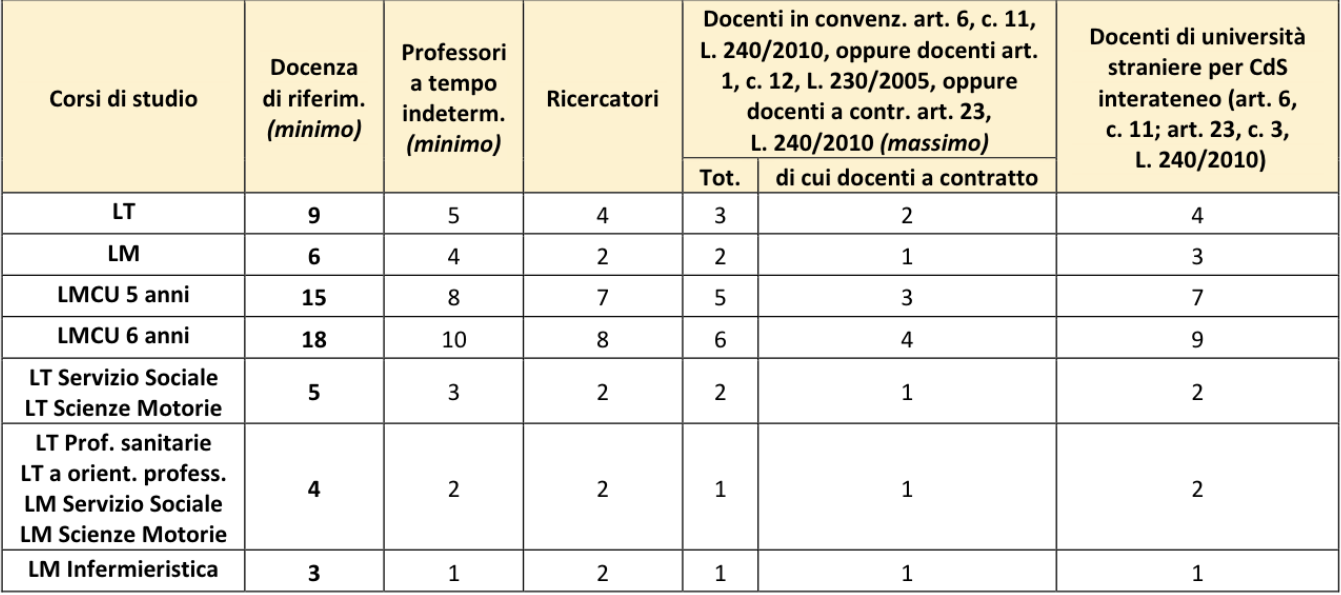
\includegraphics[width=0.8\textwidth]{images/tabella_ministeriale.png}
    \caption{Casi particolari}
    \label{fig:casi_particolari}
\end{figure}

Per fare ciò abbiamo seguito la seguente logica per ogni caso, adattandola al corso da verificare.
Prendendo come esempio la Laurea Triennale di Servizio Sociale abbiamo sostituito il codice del tipo del corso (precedente "LT") con "LTSS"
solo nelle righe dove la colonna relativa alla descrizione del corso conteneva un pattern contentente entrambe le keyworld "serviz" "social".

Dopo aver proseguito con questa serie di operazioni abbiamo ottenuto file omogenei e ben strutturati, rendendo possibile l'analisi dei dati.

\section{Answer Set Programming}\label{sec:asp}

In questa sezione approfondiamo l'organizzazione del progetto, evidenziando 
come sia stato strutturato per garantire chiarezza e modularità. 
Per facilitare l'ordine visivo e semplificare eventuali ispezioni manuali, 
il progetto è stato suddiviso in più file sorgenti, ciascuno dedicato a un 
aspetto specifico del dataset e delle regole.

Abbiamo separato i fatti e le regole in due file principali: uno dedicato 
ai docenti (Sezione~\ref*{sec:rules-docenti}) e un altro focalizzato sulle 
coperture (Sezione~\ref*{sec:rules-coperture}). Per maggiore praticità, è 
stato creato un file specifico per i docenti a contratto 
(Sezione~\ref*{sec:rules-docenti-contratto}) e un altro per i limiti 
ministeriali (Sezione~\ref*{sec:rules-ministeriale}).

Il file principale, il main, integra tutte le regole relative ai garanti, 
inclusi i vincoli e le priorità definite per l'ottimizzazione del sistema 
(Sezione~\ref*{sec:garanti}).

È importante sottolineare che tutti questi file vengono generati dinamicamente 
dal programma di preprocessing scritto in Python. Questa fase, gestita dal 
file \texttt{main.py} del preprocessing, automatizza la creazione delle regole 
e dei fatti ASP in base ai dati forniti, garantendo così una configurazione 
personalizzata e facilmente aggiornabile. 


\subsection{Docenti}\label{sec:rules-docenti}
Il file \texttt{docenti.lp} contiene una rappresentazione strutturata delle 
informazioni relative ai docenti, organizzate in diverse sezioni per garantire 
chiarezza e modularità. Questo file serve come base per definire le caratteristiche 
dei docenti e il loro SSD.

La prima parte del file definisce gli SSD disponibili, ognuno rappresentato da una 
coppia di valori: la disciplina e il livello associato (e.g., INF/01, MAT/03). Gli SSD 
sono utilizzati per verificare la compatibilità tra i docenti e i corsi di laurea.

Successivamente, vengono dichiarate le fasce contrattuali dei docenti (\texttt{td} 
per tempo determinato, \texttt{ti} per tempo indeterminato). Queste fasce sono 
utilizzate per distinguere i docenti in base alla loro tipologia di contratto,
aspetto rilevante per rispettare i requisiti ministeriali.

La sezione relativa ai docenti include l'elenco completo dei docenti, ciascuno 
identificato da una matricola unica. Per ogni docente, vengono indicate la fascia 
contrattuale e il settore scientifico disciplinare caratterizzante, che ne 
definisce il dominio di competenza. Queste informazioni sono formalizzate tramite 
il predicato \texttt{docente/4}, che associa la matricola del docente, la fascia, 
il settore disciplinare e il livello SSD.

\begin{lstlisting}[language=prolog, caption={Esempio struttura dati di \texttt{docenti.lp}.}]    
 %  SEZIONE: SSD
 ssd(inf, 1).

 %  SEZIONE: FASCIE
 fascia(td).
 fascia(ti).

 %  SEZIONE: Docenti
 %  Rossi Mario (1234), SSD caratterizzante: inf/1
 matricola_docente(1234).

 %  SEZIONE: SSD caratterizzante dei docenti
 %  Rossi Mario (1234), SSD caratterizzante: inf/1
 docente(1234, td, inf, 1) :- matricola_docente(1234), fascia(td), ssd(inf, 1).
\end{lstlisting}


\subsection{Coperture}\label{sec:rules-coperture}
Il file \texttt{coperture.lp} è fondamentale per rappresentare la struttura dei 
corsi universitari, le informazioni sui docenti assegnati e le caratteristiche 
associate a ciascun corso. Questo file contiene diverse sezioni organizzate per 
garantire chiarezza e modularità nella definizione delle informazioni.

La prima parte del file introduce i tipi di corso (\texttt{laurea/1}) e i relativi 
SSD utilizzati per caratterizzare i corsi e i docenti. Successivamente, vengono 
definiti i TAF che classificano ulteriormente gli insegnamenti.

Le informazioni sui corsi sono strutturate in due livelli: i codici identificativi 
di ciascun corso (\texttt{codice\_corso/1}) e la loro descrizione dettagliata 
tramite il predicato \texttt{corso/4}. Quest'ultimo associa il codice del corso, 
il tipo di laurea, il SSD caratterizzante e il livello del settore disciplinare.

Una parte cruciale del file riguarda la relazione tra corsi e docenti, formalizzata 
tramite il predicato \texttt{cattedra/4}. Questo predicato associa un docente 
(identificato tramite la matricola) a un corso specifico, includendo il tipo di 
laurea e il TAF relativo. 

Di seguito, un esempio rappresentativo del contenuto del file.

\begin{lstlisting}[language=prolog, caption={Esempio struttura dati di \texttt{coperture.lp}.}]    
 %  SEZIONE: Tipi di Corso
 laurea(lt).
 laurea(lm).

 %  SEZIONE: TAF
 taf(a).
 taf(b).
 taf(c).

 %  SEZIONE: Corsi
 %  INFORMATICA (3027)
 codice_corso(3027).

 %  SEZIONE: Informazioni Corsi
 corso(3027, lt, inf, 1) :- codice_corso(3027), laurea(lt), ssd(inf, 1).

 %  SEZIONE: Relazioni Corsi-Docenti
 %  Corso: 3027, Docente: Rossi Mario
 cattedra(3027, 1234, lt, b) :- codice_corso(3027), 
                                matricola_docente(1234), 
                                laurea(lt), taf(b).

\end{lstlisting}


\subsection{Docenti a contratto}\label{sec:rules-docenti-contratto}

Il file \texttt{docenti\_a\_contratto.lp} contiene informazioni relative ai docenti a 
contratto, una categoria utilizzata come risorsa di emergenza nei casi in cui i vincoli 
ministeriali non possono essere soddisfatti con i docenti a tempo determinato o 
indeterminato. Questi docenti sono identificati dalla fascia \texttt{c} e vengono 
trattati come \textit{jolly}, ovvero risorse flessibili da impiegare per garantire la 
copertura minima dei corsi universitari.

Essendo considerati come \textit{jolly}, i docenti a contratto non sono associati a 
un SSD specifico o a un corso particolare, ma possono essere assegnati liberamente per 
colmare le lacune nei corsi che non soddisfano i requisiti minimi con i docenti delle 
altre fasce. Il file \texttt{docenti\_a\_contratto.lp} è strutturato in modo minimale, 
definendo la fascia \texttt{c} e un unico predicato \texttt{jolly/1}, che indica la 
possibilità di assegnare tali docenti in modo trasversale a qualsiasi corso.

Nel modello ASP proposto, i docenti a contratto vengono inclusi come possibili garanti, 
ma il loro utilizzo è regolato e penalizzato nel processo di ottimizzazione, che vedremo
meglio nella Sezione~\ref{sec:priorita}. 

\begin{lstlisting}[language=prolog, caption={Esempio struttura dati di \texttt{docenti\_a\_contratto.lp}.}]
 %  SEZIONE: FASCIE
 fascia(c).

 jolly(1).
\end{lstlisting}


\subsection{Limiti ministeriali}\label{sec:rules-ministeriale}

Il file \texttt{ministeriale.lp} contiene i dati relativi ai requisiti ministeriali per 
ogni corso di laurea, con particolare riferimento al numero minimo di garanti richiesti 
per ciascun corso. Ogni corso ha associato un insieme di valori che determinano i vincoli 
di assegnazione dei docenti, inclusi i docenti a tempo indeterminato e tempo determinato,
e il numero massimo di docenti a contratto.

Le regole \texttt{ministeriale/5} sono calcolate dinamicamente durante la fase di 
preprocessing. In particolare, questi valori sono determinati sulla base del numero di 
studenti iscritti a ciascun corso e grazie all'applicazione della formula della \textit{W}, 
come illustrato nella Tabella~\ref{tab:formula-w}, la quale tiene conto delle specifiche 
necessità di copertura di ciascun corso. Nello specifico, la $W$ viene calcolata nel 
seguente modo:
$$
W = \frac{
        \text{Studenti iscritti al corso}
    }
    {
        \text{Massimo teorico di iscritti al corso}
    }
    - 1
$$

Di seguito un esempio della struttura del file per il corso di Informatica, per 
il quale sono richiesti almeno 9 garanti, di cui 5 a tempo indeterminato, 4 a tempo 
determinato, e un massimo di 2 docenti a contratto. 

\begin{lstlisting}[language=prolog, caption={Esempio struttura dati di \texttt{ministeriale.lp}.}]    
 %  SEZIONE: Garanti minimi per corso (codice_corso, minimo_complessivo, 
 %                                     docenti_ti, docenti_td, 
 %                                     max_docenti_contratto)
 ministeriale(3027, 9, 5, 4, 2).
\end{lstlisting} 

\begin{table}[h]
    \centering
    \renewcommand{\arraystretch}{1.5}
    \begin{tabular}{|l|c|c|}
    \hline
    \textbf{Qualifica} & \textbf{\# base} & \textbf{\# effettivo} \\
    \hline
    Docenza di riferimento & 9 & $\lfloor 9 \times (1+w) \rfloor$ \\
    \hline
    Docenti a tempo indeterminato & 5 & $\lfloor 5 \times (1+w) \rfloor$ \\
    \hline
    Docenti a contratto & 2 & $\lfloor 2 \times (1+w) \rfloor$ \\
    \hline
    \end{tabular}
    \caption{Formule per il calcolo del numero di docenti di riferimento in base alla numerosità degli studenti.}
    \label{tab:formula-w}
\end{table}

\subsection{Generazione dei garanti}\label{sec:garanti}

La generazione dei \textit{garanti} rappresenta un elemento chiave nella modellazione ASP 
sviluppata per questo progetto. In particolare, è stata posta attenzione alla distinzione 
tra i docenti appartenenti a diverse fasce contrattuali, separando i docenti 
\textbf{non a contratto} da quelli \textbf{a contratto}, i quali vengono utilizzati 
esclusivamente come risorsa di emergenza.
Inoltre, ogni docente può essere conteggiato una sola volta oppure, al massimo, essere 
assegnato a due corsi distinti con un peso pari a $0.5$ su ciascun corso. 

Per soddisfare quest'ultimo requisito, il modello ASP proposto utilizza una gestione 
basata sui pesi, i quali rappresentano il livello di impegno del docente come garante:
\begin{itemize}
    \item Un peso di \textbf{10} indica che il docente è assegnato al 100\% su un singolo corso.
    \item Un peso di \textbf{5} rappresenta un docente che divide il proprio impegno al 50\% su due corsi diversi.
\end{itemize}

\begin{lstlisting}[language=prolog, caption=Generazione dei pesi.]
% Predicati di base per definire i pesi possibili.
peso(5).
peso(10).
\end{lstlisting}

\paragraph{Docenti non a contratto.}
I docenti \textit{non a contratto}, appartenenti alle fasce \textit{tempo determinato} 
(\texttt{td}) e \textit{tempo indeterminato} (\texttt{ti}), costituiscono la base principale 
per l'assegnazione dei garanti. La regola ASP proposta genera i possibili garanti per ciascun corso, 
escludendo esplicitamente i docenti a contratto (\texttt{c}).

\begin{lstlisting}[language=prolog, caption=Generazione dei garanti non a contratto.]
Minimo{
      garante(Docente, Corso, Peso, Fascia) :
            cattedra(Corso, Docente, _, _),
            peso(Peso),
            docente(Docente, Fascia, _, _),
            fascia(Fascia),
            Fascia != c
      } :-
            ministeriale(Corso, Minimo, _, _, _).
\end{lstlisting}

In questa regola, il numero minimo di garanti per ciascun corso è regolato dal valore \texttt{Minimo} 
specificato dalla normativa ministeriale, in quanto una soluzione con un numero di garanti minore al 
minimo ministeriale verrebbe scartata, mentre il peso associato ai garanti può assumere i valori 5 o 
10, come definito dal predicato \texttt{peso/1}.

\paragraph{Docenti a contratto.}
I docenti \textit{a contratto} vengono considerati come una risorsa ausiliaria, identificati tramite 
il predicato \texttt{jolly/1}. A differenza dei docenti non a contratto, i docenti a contratto possono 
essere assegnati a qualsiasi corso, indipendentemente dall'SSD. Tuttavia, il loro utilizzo è regolato 
da un limite massimo per corso, specificato dalla normativa ministeriale, come mostrato nel frammento
di codice seguente.

\begin{lstlisting}[language=prolog, caption=Generazione dei garanti a contratto.]
{     
      garante(Docente, Corso, 10, c) :
            jolly(Docente),
            codice_corso(Corso)
}Massimo :- ministeriale(Corso, _, _, _, Massimo).
\end{lstlisting}

Questa regola garantisce che il numero di docenti a contratto utilizzati come garanti non ecceda il 
valore massimo consentito, specificato dal valore \texttt{Massimo} associato al corso.


\subsection{Vincoli}\label{sec:constraints}

I vincoli definiti in questo modello costituiscono la struttura portante del sistema, garantendo 
che le soluzioni generate siano coerenti con i requisiti ministeriali e istituzionali. 
Tutti i vincoli introdotti sono \textbf{strong}, il che significa che ogni soluzione che li 
viola viene automaticamente esclusa. 

Per garantire che ogni corso soddisfi i requisiti ministeriali, il numero di docenti assegnati 
come garanti è soggetto a controlli rigorosi. Innanzitutto, i garanti a tempo indeterminato 
(\texttt{ti}) devono essere almeno pari al minimo richiesto per ciascun corso. Allo stesso modo, 
il numero di garanti a tempo determinato (\texttt{td}) non deve superare il massimo consentito. 
Questi vincoli assicurano che il modello rispetti le linee guida istituzionali senza 
sovraccaricare un'unica tipologia di docenti.

\begin{lstlisting}[language=prolog, caption={Vincoli su garanti a tempo indeterminato e determinato.}]
 :- conta_garanti_indeterminato(Corso, Numero),
      ministeriale(Corso, Minimo, Minimo_ind, _, _),
      Numero < Minimo_ind.

 :- conta_garanti_determinato(Corso, Numero),
      ministeriale(Corso, _, _, Massimo_det, _),
      Numero > Massimo_det.
\end{lstlisting}

Il modello include vincoli che controllano i pesi assegnati ai garanti. La somma totale dei 
pesi per ciascun corso deve essere almeno 10 volte il numero minimo di garanti richiesti, 
poiché un docente è considerato \textit{effettivo} solo se il suo peso totale raggiunge il valore 
massimo di 10. Inoltre, tale somma deve essere un multiplo di 10 per garantire la coerenza 
nell'assegnazione del garante stesso.

\begin{lstlisting}[language=prolog, caption={Vincoli sui pesi assegnati ai garanti.}]
 :- somma_pesi_corso(Corso, Somma),
      ministeriale(Corso, Minimo, _, _, _),
      Min = 10 * Minimo,
      Somma < Min.

 :- somma_pesi_corso(Corso, Somma),
      Modulo = Somma \ 10,
      Modulo != 0.
\end{lstlisting}

Per evitare conflitti e garantire una distribuzione equa del carico di lavoro, ogni docente 
può essere associato ad un massimo di due corsi, ma con una somma totale di pesi non superiore 
a 10. Inoltre, un docente non può essere associato allo stesso corso con pesi differenti che, 
sommati, superano 10.

\begin{lstlisting}[language=prolog, caption={Vincoli sulla distribuzione dei pesi per docente.}]
 :- garante(Docente, Corso1, Peso1, Fascia),
      garante(Docente, Corso2, Peso2, Fascia),
      Somma = Peso1 + Peso2,
      Somma > 10,
      Fascia != c,
      Corso1 != Corso2.

 :- garante(Docente, Corso1, Peso1, Fascia),
      garante(Docente, Corso1, Peso2, Fascia),
      Somma = Peso1 + Peso2,
      Somma > 10,
      Fascia != c,
      Peso1 != Peso2.
\end{lstlisting}

Per mantenere la coerenza tra i garanti e gli SSD caratterizzanti di ciascun corso, almeno 
il 50\% dei garanti deve afferire all'SSD del corso. In caso contrario, la soluzione viene esclusa.

\begin{lstlisting}[language=prolog, caption={Vincolo sui garanti afferenti al SSD caratterizzante.}]
 :- numero_garanti_che_afferiscono(Aff, Corso),
      numero_garanti_di_riferimento(Tot, Corso),
      2 * Aff <= Tot.
\end{lstlisting}

Infine, il numero totale di docenti a contratto assegnati a ciascun corso non può superare il 
limite massimo specificato dai requisiti ministeriali.

\begin{lstlisting}[language=prolog, caption={Vincolo sul numero massimo di docenti a contratto.}]
 :- jolly_per_corso(Corso, Numero),
      ministeriale(Corso, _, _, _, Massimo_numero_docenti_a_contratto),
      Numero > Massimo_numero_docenti_a_contratto.
\end{lstlisting}






\subsection{Gestione delle priorità}\label{sec:priorita}
La gestione delle priorità è stata un aspetto fondamentale nel nostro progetto, poiché 
miravamo a rispettare scrupolosamente i vincoli ministeriali, garantendo al contempo 
flessibilità per gestire situazioni particolari in cui tali vincoli non fossero 
pienamente soddisfacibili.

Per organizzare le priorità dei garanti, abbiamo deciso di basarci, in seguito ad un 
colloquio con l'ufficio didattico, principalmente sulla loro tipologia contrattuale. 
Il nostro obiettivo era quello di massimizzare l'impiego di docenti a tempo determinato 
(i.e., ricercatori) e a tempo indeterminato (i.e., professori associati e ordinari), prima 
di ricorrere ai docenti a contratto, che sono utilizzati solo quando strettamente necessario. 
Per ottimizzare la gestione, abbiamo preferito che i docenti assumessero il ruolo di 
garanti per un solo corso, evitando situazioni in cui un docente fosse impegnato come 
garante per più corsi contemporaneamente al 50\%.

\begin{lstlisting}[language=prolog, caption=Gestione delle priorità dei docenti.]
 % Docenti a tempo determinato (ricercatori)
 #maximize { 50 : garante(_, _, _, td) }.

 % Docenti a tempo indeterminato
 #maximize { 40 : garante(_, _, _, ti) }.

 % Docenti a contratto
 #maximize { 32 : garante(_, _, _, c) }.

 % Docenti con peso 10
 #maximize { 25 : garante(_, _, Peso, _), Peso = 10 }.

 % Minimizzare i docenti con peso 5
 #minimize { 100, Docente : garante(Docente, _, Peso, _), Peso = 5 }.
\end{lstlisting}

Inoltre, abbiamo dato priorità ai docenti che insegnano corsi fondamentali per i 
corsi di laurea, distinguendo tra gli insegnamenti di base, identificati dal TAF A, 
e gli insegnamenti caratterizzanti, identificati dal TAF B.

\begin{lstlisting}[language=prolog, caption=Gestione delle priorità del TAF.]
 % Garanti che hanno insegnamenti di base
 #maximize { 25 : garante(Docente, Corso, _, _), 
                  cattedra(Corso, Docente, _, TAF), 
                  TAF = a}.

 % Garanti che hanno insegnamenti caratterizzanti
 #maximize { 18 : garante(Docente, Corso, _, _), 
                  cattedra(Corso, Docente, _, TAF), 
                  TAF = b}.

 % Garanti che hanno insegnamenti affini
 #maximize { 10 : garante(Docente, Corso, _, _), 
                  cattedra(Corso, Docente, _, TAF), 
                  TAF = c}.
\end{lstlisting}

Per ottimizzare l'assegnazione dei garanti in base alla loro competenza, sono stati 
privilegiati i docenti il cui l'SSD corrisponde a quello caratterizzante del corso.
In questo modo, ci siamo assicurati che i garanti siano adeguatamente allineati con 
le competenze richieste dai corsi.

\begin{lstlisting}[language=prolog, caption=Preferenza dei garanti con macrosettore coerente a quello del corso.]
% Ottimizzare i garanti con SSD caratterizzante
#maximize { 20 : garante(Docente, Corso, _, _), 
                 docente(Docente, _, SettoreSSD, _), 
                 corso(Corso, _, SettoreSSD, _) }.
\end{lstlisting}

Infine, per mantenere l'equilibrio tra la qualità e l'efficacia del sistema, abbiamo 
minimizzato il numero di garanti assegnati a ciascun corso, penalizzando le situazioni 
in cui il numero di garanti supera il minimo richiesto. Questo vincolo ci ha permesso 
di ottimizzare le risorse, evitando l'assegnazione di più docenti di quanto fosse necessario.

\begin{lstlisting}[language=prolog, caption=Minimizzazione dei garanti per corso di laurea.]
% Minimizzo il numero di garanti per ogni corso
#minimize { Penalita : garanti_per_corso(Corso, Numero),
                       Penalita = Numero * 10 }.
\end{lstlisting}


\section{Esempio giocattolo}
\label{sec:esempio-giocattolo}

\section{Validazione della soluzione proposta}
\label{sec:expval}

Per testare l'efficacia e la correttezza del modello sviluppato, è stato creato un esempio 
giocattolo basato sui corsi di laurea in Informatica (LT) e Scienze Informatiche (LM). 
Questo dataset ridotto è stato progettato per verificare la capacità del modello ASP di 
generare soluzioni valide, rispettando i vincoli definiti e implementando correttamente 
le ottimizzazioni.

I dati di input per il modello sono stati generati attraverso un comando Python, che ha 
prodotto i file necessari contenenti i fatti relativi ai docenti, alle coperture, ai 
docenti a contratto e ai limiti ministeriali.

\begin{lstlisting}[language=bash]
 python3 main.py --3027 --5069
\end{lstlisting}

Una volta generati i file, l'analisi è stata eseguita utilizzando Clingo.

\begin{lstlisting}[language=bash]
 clingo -n 15 --parallel-mode 8 --time-limit=180 lp/* main.lp
\end{lstlisting}

Il modello ha prodotto una soluzione ottima in un \textit{centesimo di un secondo}, 
dimostrando tempi di computazione estremamente brevi. Per il corso di Informatica 
(codice: 3027) sono stati assegnati 9 garanti in conformità ai requisiti. Per il corso di 
Scienze Informatiche (codice: 5069) sono stati assegnati 6 garanti, sempre in conformità ai 
requisiti

È stata inoltre verificata la coerenza tra i garanti assegnati e gli SSD caratterizzanti, 
con 5 docenti afferenti per Informatica e 4 per Scienze Informatiche.

\subsection{Dataset ridotto: Dipartimento SMFI}
\label{sec:-dataset-dipartimento-smfi}

Per valutare la scalabilità del modello, è stato eseguito un test utilizzando un dataset 
ridotto relativo al Dipartimento di Scienze Matematiche, Fisiche e Informatiche (SMFI), 
comprendente sei corsi di studio. Anche in questo caso, i file di input sono stati generati 
tramite Python.

\begin{lstlisting}[language=bash]
 python3 main.py --3027 --5069 --3026 --5036 --3030 --5037
\end{lstlisting}

L'analisi è stata eseguita con Clingo utilizzando lo stesso comando precedentemente 
indicato. Il modello ha dimostrato di poter gestire un numero maggiore di corsi, producendo 
soluzioni valide in tempi brevi. In questo caso, il tempo di computazione è stato di circa 
\textit{due secondi} per ottenere la soluzione ottimale.

Durante il test, è stata utilizzata la configurazione che prevede solo pesi pari a 10, al 
fine di ridurre la complessità computazionale. Tuttavia, il modello supporta anche l'opzione 
di pesi pari a 5, che, pur aumentando significativamente i tempi di computazione, offre 
maggiore flessibilità nella generazione delle soluzioni.




\subsection{Dataset grande (tutti i dipartimenti)}
\label{sec:dataset-tutti-dipartimenti}
\section{Conclusioni}
\label{sec:conclusion}


\textit{Acknowledgments} \\Questo progetto è stato realizzato nel corso di Programmazione Dichiarativa (a.a. 2024-25), presso l'Università degli Studi di Parma.\\

\hfill

\break
\printbibliography

\end{document}
